\section{Résultats et livrables entreprise}
Comme les attentes initiales de Panorama Performance s’approchaient trop d’une application complète (plus que d’une POC) et que nous avions trop peu de temps pour développer toutes les fonctionnalités que l’équipe souhaitait, nous avons dû choisir un certain nombre de fonctionnalités à implémenter. Notre objectif était de développer une POC, la plus simple possible, mais munie des fonctionnalités principales, afin de voir si ce projet était réellement viable et pourrait être au minimum équivalent à la version papier. \\

Nous avons estimé les différentes options afin d’effectuer cette digitalisation, et nous avons retenu que la faire réaliser par un freelance était le plus rentable. Cependant, sur le long terme, il vaudrait mieux embaucher un développeur Full Stack au sein de l’entreprise afin de pouvoir améliorer la solution et corriger les éventuels problèmes.\\

Nous avons également réalisé une partie économique de ce projet afin de pouvoir voir si ce projet était rentable grâce à la création d’un abonnement annuel. Nous avons donc estimé que ce projet l’était, avec un retour sur investissement sur 3 ans après le déploiement de la solution.\\

 Suite à la phase de test réalisé le mercredi 2 juin en salle E004, Panorama Performance nous a annoncé vouloir pousser le développement pour obtenir un MVP. Ils présenteront ensuite l'application à leurs clients les plus réguliers, et en fonction de leurs retour (usabilité, simplicité, besoin, \dots) ils lanceront, ou non, le développement final.\\
 
 \begin{figure}[!h]
     \centering
     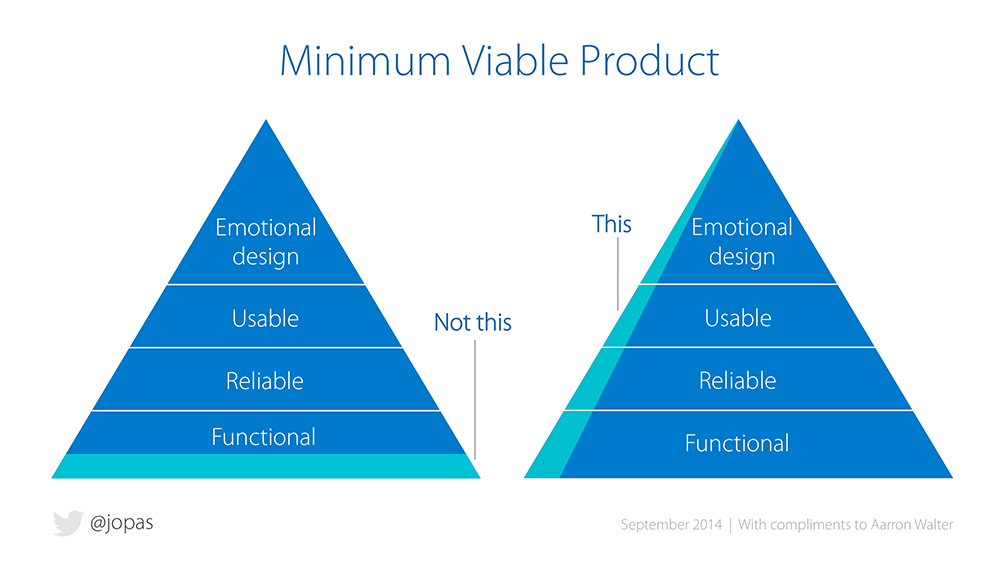
\includegraphics[scale=0.3]{img/MVP.png}
     \caption{Principe du Minimum Viable Product}
     \label{fig:my_label}
 \end{figure}

La dernière semaine du projet va également être l'occasion de commenter le code pour permettre sa transmission à une possible nouvelle équipe de développement. De cette manière, le projet n'aura pas à repartir de zéro. Le code ainsi que l'accès à la base de données seront en effet fournis à Panorama Performance à la fin de ce projet Activ'ESAIP, de cette manière, ils pourront présenter la version qui est déjà disponible en ligne, mais également en modifier certaines fonctionnalités ou en ajouter.